% Options for packages loaded elsewhere
\PassOptionsToPackage{unicode}{hyperref}
\PassOptionsToPackage{hyphens}{url}
%
\documentclass[
  ignorenonframetext,
  aspectratio=169]{beamer}
\usepackage{pgfpages}
\setbeamertemplate{caption}[numbered]
\setbeamertemplate{caption label separator}{: }
\setbeamercolor{caption name}{fg=normal text.fg}
\beamertemplatenavigationsymbolsempty
% Prevent slide breaks in the middle of a paragraph
\widowpenalties 1 10000
\raggedbottom
\setbeamertemplate{part page}{
  \centering
  \begin{beamercolorbox}[sep=16pt,center]{part title}
    \usebeamerfont{part title}\insertpart\par
  \end{beamercolorbox}
}
\setbeamertemplate{section page}{
  \centering
  \begin{beamercolorbox}[sep=12pt,center]{part title}
    \usebeamerfont{section title}\insertsection\par
  \end{beamercolorbox}
}
\setbeamertemplate{subsection page}{
  \centering
  \begin{beamercolorbox}[sep=8pt,center]{part title}
    \usebeamerfont{subsection title}\insertsubsection\par
  \end{beamercolorbox}
}
\AtBeginPart{
  \frame{\partpage}
}
\AtBeginSection{
  \ifbibliography
  \else
    \frame{\sectionpage}
  \fi
}
\AtBeginSubsection{
  \frame{\subsectionpage}
}
\usepackage{lmodern}
\usepackage{amssymb,amsmath}
\usepackage{ifxetex,ifluatex}
\ifnum 0\ifxetex 1\fi\ifluatex 1\fi=0 % if pdftex
  \usepackage[T1]{fontenc}
  \usepackage[utf8]{inputenc}
  \usepackage{textcomp} % provide euro and other symbols
\else % if luatex or xetex
  \usepackage{unicode-math}
  \defaultfontfeatures{Scale=MatchLowercase}
  \defaultfontfeatures[\rmfamily]{Ligatures=TeX,Scale=1}
\fi
\usetheme[]{Frankfurt}
\usecolortheme{beaver}
% Use upquote if available, for straight quotes in verbatim environments
\IfFileExists{upquote.sty}{\usepackage{upquote}}{}
\IfFileExists{microtype.sty}{% use microtype if available
  \usepackage[]{microtype}
  \UseMicrotypeSet[protrusion]{basicmath} % disable protrusion for tt fonts
}{}
\makeatletter
\@ifundefined{KOMAClassName}{% if non-KOMA class
  \IfFileExists{parskip.sty}{%
    \usepackage{parskip}
  }{% else
    \setlength{\parindent}{0pt}
    \setlength{\parskip}{6pt plus 2pt minus 1pt}}
}{% if KOMA class
  \KOMAoptions{parskip=half}}
\makeatother
\usepackage{xcolor}
\IfFileExists{xurl.sty}{\usepackage{xurl}}{} % add URL line breaks if available
\IfFileExists{bookmark.sty}{\usepackage{bookmark}}{\usepackage{hyperref}}
\hypersetup{
  pdftitle={Applications of Tissue Culture for Crop Improvement},
  pdfauthor={Deependra Dhakal},
  hidelinks,
  pdfcreator={LaTeX via pandoc}}
\urlstyle{same} % disable monospaced font for URLs
\newif\ifbibliography
\setlength{\emergencystretch}{3em} % prevent overfull lines
\providecommand{\tightlist}{%
  \setlength{\itemsep}{0pt}\setlength{\parskip}{0pt}}
\setcounter{secnumdepth}{-\maxdimen} % remove section numbering
\usepackage{booktabs}
\usepackage{longtable}
\usepackage{array}
\usepackage{multirow}
\usepackage{wrapfig}
\usepackage{float}
\usepackage{colortbl}
\usepackage{pdflscape}
\usepackage{tabu}
\usepackage{threeparttable}
\usepackage{threeparttablex}
\usepackage[normalem]{ulem}
\usepackage{makecell}
\usepackage{xcolor}
\usepackage{tikz} % required for image opacity change
\usepackage[absolute,overlay]{textpos} % for text formatting

% this font option is amenable for beamer
\setbeamerfont{caption}{size=\tiny}
\setbeamerfont{footnote}{size=\tiny}

\setbeamertemplate{footline}[page number] % insert page number in footline
\newlength{\cslhangindent}
\setlength{\cslhangindent}{1.5em}
\newenvironment{cslreferences}%
  {\setlength{\parindent}{0pt}%
  \everypar{\setlength{\hangindent}{\cslhangindent}}\ignorespaces}%
  {\par}

\title{Applications of Tissue Culture for Crop Improvement}
\author{Deependra Dhakal}
\date{}
\institute{College of Natural Resource Management, Tikapur,
Kailali \and Agriculture and Forestry University}

\begin{document}
\frame{\titlepage}

\begin{frame}[allowframebreaks]
  \tableofcontents[hideallsubsections]
\end{frame}
\hypertarget{organ-culture}{%
\section{Organ culture}\label{organ-culture}}

\begin{frame}{}
\protect\hypertarget{section}{}
\begin{itemize}
\tightlist
\item
  Root: excised radical tip.
\item
  Leaf: Immature young leaf of shoot apex.
\item
  Shoot tip: 0.1-1.0 mm terminal portion of shoot.
\item
  Meristem : \textless{} 0.1 mm.
\item
  Flower: excised floral bud.
\item
  Ovary : isolated ovary.
\item
  Ovule culture
\item
  Embryo culture
\end{itemize}
\end{frame}

\hypertarget{double-haploids}{%
\section{Double haploids}\label{double-haploids}}

\begin{frame}{}
\protect\hypertarget{section-1}{}
\begin{itemize}
\tightlist
\item
  Haploids are individuals possessing a single set of chromosomes of the
  species (n; number of chromosomes in a gamete).
\item
  DHs were first reported in 1920 in a dwarf cotton plant. Later in
  \emph{Datura stramonium} and \emph{Nicotiana tabacum}.
\item
  Haploid induction and double haploid generation can be achieved by:

  \begin{itemize}
  \tightlist
  \item
    Haploid inducing gene
  \item
    Anther/microspore culture
  \item
    Interspecific cross
  \end{itemize}
\item
  No direct benefits to cultivation -- less vigorous, susceptible to
  biotic and abiotic stresses.
\item
  In plant breeding, they are prized because they are completely
  \textbf{homozygous} for all loci and this phenomena can be obtained in
  very short period of time. Self pollinating population require 5-8
  generations of selfing in order to achieve desired level of
  homozygosity.
\end{itemize}
\end{frame}

\begin{frame}{}
\protect\hypertarget{section-2}{}
\[
\text{Homozygosity}_n = 1 - \left(\frac{1}{2}\right)^n
\]

\begin{table}

\caption{\label{tab:homozygosity-accumulation}Percentage of homozygosity and number of self pollinations needed to obtain inbred lines in a traditional breeding program of autogamous species.}
\centering
\begin{tabular}[t]{rl}
\toprule
Generations & Homozygosity\\
\midrule
1 & 50.00\%\\
2 & 75.00\%\\
3 & 87.50\%\\
4 & 93.75\%\\
5 & 96.88\%\\
\addlinespace
6 & 98.44\%\\
7 & 99.22\%\\
\bottomrule
\end{tabular}
\end{table}
\end{frame}

\begin{frame}{Haploid production}
\protect\hypertarget{haploid-production}{}
\begin{enumerate}
\tightlist
\item
  Selection of parents
\item
  Crossing
\item
  F1 plants are advanced to F2 for segregation (not necessary if parents
  with haploid inducer genes are used in crossing or if F1 gametes are
  available for culture)
\item
  F1/F2 are used as source of variability for DH lines
  production\footnote<.->{Simulation studies have shown that haploids
    from F2 plants may be more efficient due to greater segregation and
    opportunity of linkage breakages with the \(\bigotimes\)}.
\end{enumerate}

\begin{itemize}
\tightlist
\item
  Of several methods available,

  \begin{itemize}
  \tightlist
  \item
    Anther culture is efficient in barley, wheat, and brassicas, but not
    as successful in soybean, common beans and oats
  \item
    Haploid inducing lines are commonly used in maize
  \end{itemize}
\item
  DH plants of over 250 species have been successfully reproduced using
  anther culture.
\end{itemize}
\end{frame}

\begin{frame}{Haploid plants from anther culture}
\protect\hypertarget{haploid-plants-from-anther-culture}{}
\begin{itemize}
\tightlist
\item
  Gametic cell may be diverted from its normal organogenic route to
  develop a somatic cell, via embryogenesis or organogenesis, is
  responsible for haploid production.
\item
  Culture of anthers or isolated micropsores to produce haploid plants
  is known as anther culture or microspore culture.
\item
  Embryos can be produced via a callus phase or be a direct
  recapitulation of the developmental stages characteristic of zygotic
  embryos.
\item
  late uninucleate to early binucleate microspores are the best explants
  for embryogenesis.
\item
  Somatic embryos develop into haploid plants.
\end{itemize}
\end{frame}

\begin{frame}{}
\protect\hypertarget{section-3}{}
\begin{itemize}
\tightlist
\item
  Chromosome doubling can be further used to produce doubled haploids
  (homozygous).
\item
  In addition, haploid embryos are used in mutant isolation, gene
  transfer, studies of storage product biochemistry, and physiological
  aspects of embryo maturation.
\end{itemize}

Flowdiagram ?
\end{frame}

\begin{frame}{Procedure for anther culture}
\protect\hypertarget{procedure-for-anther-culture}{}
\begin{itemize}
\tightlist
\item
  Take young flower buds with immature anthers. Wash the buds. Surface
  sterilise and rinse with sterile water.
\item
  Transfer the flower buds into a beaker containing basal media (50
  anthers of tobacco in 10 ml media).
\item
  Take one anther and crush in acetocarmine to test the stage of pollen.
  If found good, separate each anther from filament.
\item
  Discard immature, overmature and injured anthers.
\item
  Squeeze out microspores in pressing them against the side of beaker
  with a glass rod.
\item
  Remove anther tissue debris by filtering through nylon sieve (pore
  size \(40\mu\) for tobacco and \(100\mu\) for maize). Filter again to
  obtain larger and viable microspores.
\item
  Centrifuse the pollen suspension at low speed for 5 minutes.
\end{itemize}
\end{frame}

\begin{frame}{}
\protect\hypertarget{section-4}{}
\begin{itemize}
\tightlist
\item
  Inoculate anthers horizontally on nutrient medium (liquid, solid) by
  pipetting. Medium density for tobaccoo is \(10^3-10^4\)
  microspores/ml.
\item
  In case of Brassica, microspore is used for dissecting out the
  anthers. In case of cereals, spikes are harvested at uninucleate stage
  of microspore and then surface sterilise.
\item
  Place 10-20 anthers in a 6 cm petri dishes.
\item
  Seal each petri dish containing anther/microspores and medium with
  parafilm to avoid dehydration.
\item
  If anthers are cultured in liquid medium then 50 anthers can be
  cultured in 10 ml of liquid.
\item
  Incubate and observe.
\item
  Shoots/plantlets (3-5 cm) transfer to another medium.
\end{itemize}
\end{frame}

\begin{frame}{Embryo culture/rescue}
\protect\hypertarget{embryo-culturerescue}{}
\begin{itemize}
\tightlist
\item
  Some species produce sterile seeds that fail to germinate. This
  infertility can result from incomplete embryo development, mutations
  in structures covering the embryos resulting in their death, or a type
  of recalcitrant dormancy for which no method of breaking dormancy has
  been developed.
\item
  Embryos are isolated from immature ovules or seeds and are cultured
  \emph{in vitro}.
\item
  Embryo \textbf{rescue} also finds use in the production of
  interspecific hybrids between inviable crosses, whose seeds are
  discarded because of their inability to germinate.
\item
  Generally, embryo culture goes hand in hand with in vitro control of
  pollination and fertilization to ensure hybrid production.
\item
  Immature embryos can be used to produce embryogenic callus and somatic
  embryos or direct somatic embryos.
\end{itemize}
\end{frame}

\begin{frame}{Embryo rescue: Application}
\protect\hypertarget{embryo-rescue-application}{}
\footnotesize

\begin{itemize}
\tightlist
\item
  Genes for tolerance/resistance to biotic or abiotic stresses have been
  lost because of the intense process of domestication.
\item
  Most frequently breeders resort to wild species to isolate new
  tolerance and resistance genes.
\item
  Although sexual crossing between different species is possible, in
  gamete fusion and embryo formation, \textbf{embryo abortion} (because
  of endosperm malformation) as a post-zygotic barrier is common.
\item
  Embryo rescue in culture media (that provides all the nutritional
  requirements to replace the endosperm function of nourishing the
  embryo) promotes normal development, enabling the generation of
  interspecific hybrids and in some cases hybrids between different
  families.
\item
  Depending on the developmental stage, the embryo should require only
  inorganic nutrients and a carbohydrate source in the culture medium,
  although supplementation with growth regulators, antioxidants,
  vitamins, and other substances is required for very young embryos.
\end{itemize}
\end{frame}

\begin{frame}{}
\protect\hypertarget{section-5}{}
\footnotesize

\begin{itemize}
\tightlist
\item
  Zygotic embryo culture method has been used successfully in palm
  trees, demonstrated by the increased germination rate, plant
  uniformity, and conversion of viable seedlings in species including
  \emph{Cocos nucifera} (Aké et al. 2007), and \emph{Hyophorbe
  lagenicaulis} (Sarasan, Ramsay, and Roberts 2002).
\item
  An experiment evalutated effect of nutrition supplement on \emph{in
  vitro} germination of macauba palm ( \emph{Acrocomia aculeata})
  seedlings, which take approximately 2 years to germinate in nature.

  \begin{itemize}
  \tightlist
  \item
    Embryos were excised and were inoculated into test tubes containing
    15 mL of MS culture medium at 50 and 100\% concentrations of mineral
    salts, supplemented with coconut water (0, 50, 100, and 150
    \(mL L^{-1}\)). The cultures were maintained in a growth room at
    approximately \(42 W m^{-2}\) irradiance, \(25\pm 2^\circ C\), and a
    16-hour photoperiod.
  \item
    Higher percentage of embryo germination was observed at 60 days in
    the MS medium at the original concentration of salts (95.6\%). The
    growth and conversion of viable or normal seedlings that were
    acclimatized required MS culture medium containing half the salt
    concentration supplemented with \(50 mL L^{-1}\) coconut water.
  \end{itemize}
\end{itemize}
\end{frame}

\begin{frame}{Interspecific hybridization for DH generation}
\protect\hypertarget{interspecific-hybridization-for-dh-generation}{}
\begin{itemize}
\tightlist
\item
  Successfully carried out in potato, alfalfa, brassica, wheat, oat,
  triticale and strawberry.
\item
  In wheat, spikelets of greenhouse grown plants are emasculated.
\item
  Three days later, artificial pollination (generally during morning) is
  done using maize pollen. Pollination may be repeated the later day to
  improve the success.
\item
  Maize pollen type/source genotype determines frequency of embryo and
  caryopsis formation.
\item
  \(2,4-D\) and \(Ag NO_3\) are applied 24 hours after second
  pollination.
\item
  Immature embryos are rescued 16-18 days after pollination, and
  transferred to P2 medium for \emph{in vitro} culture. Haploid plant
  can grow up to the period of chromosome duplication in this medium.
\item
  The development of an individual from unfertilized ovules is called
  parthenogenesis. Frequently, parthenogenesis occurs \emph{in vivo} and
  in this case is named polyembriony, as in citrus.
\end{itemize}
\end{frame}

\begin{frame}{}
\protect\hypertarget{section-6}{}
\begin{figure}
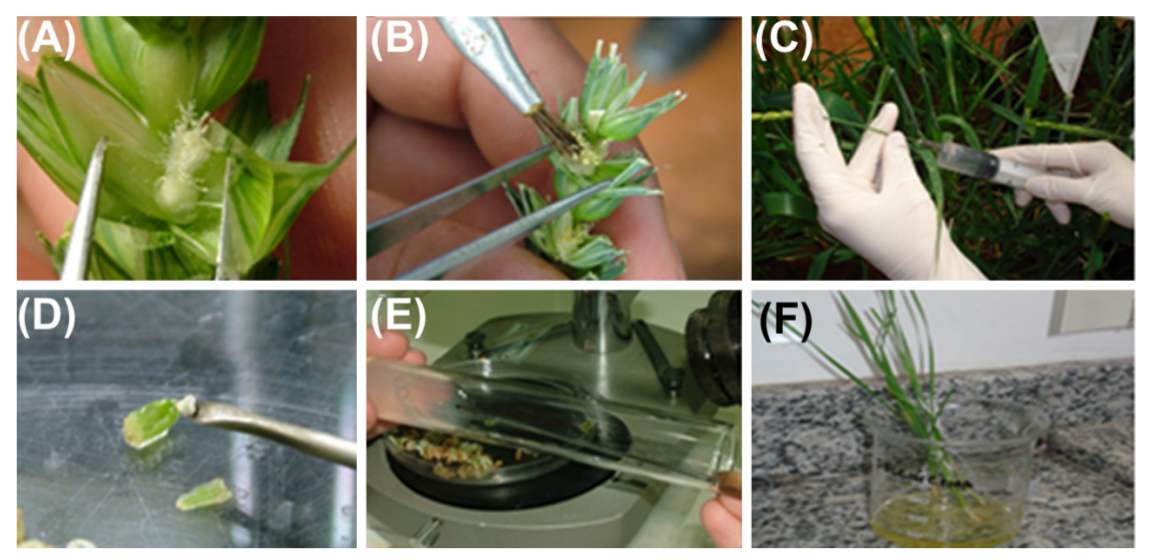
\includegraphics[width=0.6\linewidth]{../images/wheat-embryo-rescue} \caption{\textbf{Wide cross}. (A) Emasculation of wheat plants; (B) Pollination with maize pollen; (C) Application of 2,4-D and AgNO3 solution; (D) Embryo rescue; (E) Transfer to tissue culture; and (F) Double-haploid plant produced.}\label{fig:wheat-embryo-rescue-wide-hybridization}
\end{figure}
\end{frame}

\begin{frame}{Genetics of haploidization}
\protect\hypertarget{genetics-of-haploidization}{}
\begin{itemize}
\tightlist
\item
  Depending on the incompatibility of the parent genome, one of the
  genomes (usually male parent) is eliminated producing an haploid
  embryo parthenogenically.

  \begin{itemize}
  \tightlist
  \item
    Androgenetic haploid (generally induced by W23 -- efficiency ranges
    0-2\%)
  \item
    Gynogenetic haploid (generally induced by Stock 6 -- efficiency
    ranges 1-2\%)
  \end{itemize}
\item
  Androgenetic haploids are known to have gametofitic indeterminate (ig)
  mutation.
\item
  Haploid inducing lines are mostly adapted to temperate climates.
\item
  Genome elimination usually follows several of the following incidents:

  \begin{itemize}
  \tightlist
  \item
    there is no perfect pairing (spatial separation) of chromosomes of
    the two species during division
  \item
    faulty kinetochore/spindle fiber interaction
  \item
    asynchronous cycles lead to production of micronuclei, which hold
    the chromosomes isolated that otherwise would have migrated to the
    poles
  \item
    ``actual nucleus'' recognizes chromosomes as foreign DNA and cause
    their heterochromatinization and degradation.
  \item
    over several cycles of mitosis, complete chromosome elimination is
    achieved
  \end{itemize}
\end{itemize}
\end{frame}

\begin{frame}{Identification of haploids}
\protect\hypertarget{identification-of-haploids}{}
\begin{figure}
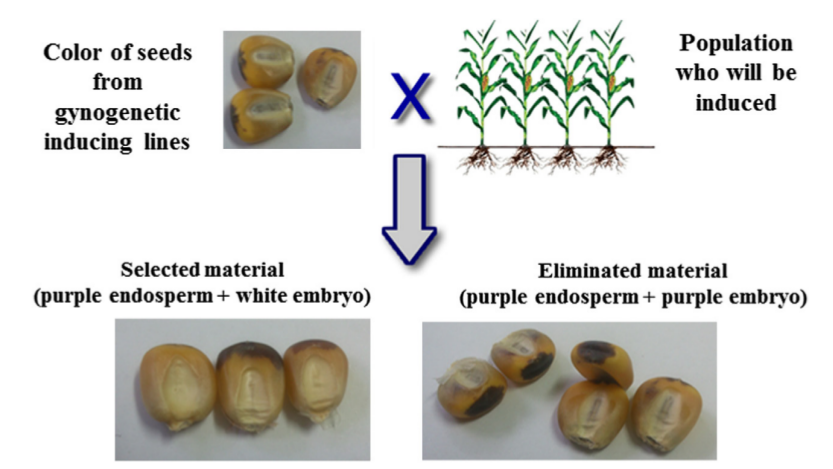
\includegraphics[width=0.7\linewidth]{../images/gynogenetic-haploid-identification} \caption{Morphological marker for seed color to identify haploids}\label{fig:gynogenetic-haploid-identification}
\end{figure}
\end{frame}

\begin{frame}{Production of doubled-haploids}
\protect\hypertarget{production-of-doubled-haploids}{}
\begin{itemize}
\tightlist
\item
  Colchicine is a mitotic inhibitor commonly used in chromosome
  duplication and also as a pre treatment for microscope slide
  preparation.

  \begin{itemize}
  \tightlist
  \item
    Bounds to the tubulin and inhibits the formation of microtubules
    that are part of the fuse fibers, avoiding the migration of the
    chromosomes.
  \end{itemize}
\item
  Stongly carcinogenic! (Alternatives are: dinitroaniline group, such as
  trifluraline and pendimethalin)
\end{itemize}
\end{frame}

\begin{frame}{}
\protect\hypertarget{section-7}{}
\begin{itemize}
\tightlist
\item
  In haploid maize duplication:

  \begin{itemize}
  \tightlist
  \item
    seeds are germinated in a moistened germination paper
  \item
    after radicle emergence small cut is made on seedling coleoptile for
    better colchicine inifiltration
  \item
    Colchicine is used at 0.06\% concentration along with 0.5 to 0.75\%
    of DMSO (dimethyl sulfoxide), seedlings are left drenched in the
    solution for 12 to 17 hours.
  \item
    After this treatment the roots are dried and transplanted to trays
    with a substrate of 1:1 of soil and vermiculite.
  \item
    plants are acclimated
  \item
    about 30\% of the haploid plants treated with colchicine may be self
    pollinated to set 100\% homozygous seeds.
  \end{itemize}
\end{itemize}
\end{frame}

\hypertarget{meristem-culture-for-virus-free-plants}{%
\section{Meristem culture for virus free
plants}\label{meristem-culture-for-virus-free-plants}}

\begin{frame}{Meristem culture for virus free plants}
\begin{itemize}
\tightlist
\item
  For the production of pathogen-free plants
\item
  Apical meristem tips is used (hence, aka. meristem culture, meristem
  tip culture, or shoot tip culture)
\item
  The apical meristem is usually a dome of tissue located at the extreme
  tip of a shoot and measures 0.1 mm in diameter and 0.25-0.3 mm in
  length. The apical meristem together with one or three young leaf
  primordial measuring 0.1-0.5 mm constitutes the shoot apex
\item
  Meristem culture in combination with thermotherapy has resulted in
  successful production of virus-free plants.
\item
  Culture involves the development of an already existing shoot apical
  meristem and the regeneration of adventitious roots.
\item
  Usually, 5-10 mm shoot apices containing the shoot meristem along with
  several leaf primordia are used.
\end{itemize}
\end{frame}

\begin{frame}{}
\protect\hypertarget{section-8}{}
\begin{itemize}
\tightlist
\item
  Benefits of meristem culture:

  \begin{itemize}
  \tightlist
  \item
    Rate of cell division is high than virus multiplication.
  \item
    High metabolic activity, No virus replication.
  \item
    No vascular system, no movement of viruses.
  \item
    Endogenous auxin level high, inhibit virus multiplication.
  \end{itemize}
\end{itemize}
\end{frame}

\begin{frame}{Procedure for meristem culturing}
\protect\hypertarget{procedure-for-meristem-culturing}{}
\small

\begin{itemize}
\tightlist
\item
  Selection

  \begin{itemize}
  \tightlist
  \item
    Take apical meristematic dome or apical dome with leaf primordial by
    applying V-shaped cut with a sterised knife and cut is applied
    0.3-0.5 mm below the tip of dome. (0.3 -- 0.5 mm: virus free, less
    than 2 cm: contamination but survival/success rate is high)
  \end{itemize}
\item
  Culture establishment; According to Murashige, there are 3 stages of
  cultures to be needed

  \begin{itemize}
  \tightlist
  \item
    Stage I: culture establishment stage: supplemented with cytokinin,
    if large sized explant used, supply auxin (0.45-10 micro mole).
  \item
    Stage II: axillary shoot proliferation is followed. Supply high
    level of cytokinin (4.5 -- 25 micro mole)
  \item
    Stage III: de novo regeneration of adventitious roots from the
    shoots obtained at stage II
  \item
    In vitro produced shoots of sufficient length are cut and placed on
    another medium containing high level of auxins and low cytokinin at
    stage III.
  \end{itemize}
\end{itemize}
\end{frame}

\begin{frame}{}
\protect\hypertarget{section-9}{}
\begin{itemize}
\tightlist
\item
  Growing

  \begin{itemize}
  \tightlist
  \item
    Temperature should be \(20-28^\circ C\) to \(24-26^\circ C\).
  \item
    Light duration: 16 day hour and 8 night hour.
  \item
    Light intensity: 1-10 k lux.
  \item
    Relative humidity
  \item
    Oxygen
  \end{itemize}
\end{itemize}
\end{frame}

\hypertarget{somatic-hybridizationprotoplast-fusion}{%
\section{Somatic hybridization/Protoplast
fusion}\label{somatic-hybridizationprotoplast-fusion}}

\begin{frame}{}
\protect\hypertarget{section-10}{}
\begin{itemize}
\tightlist
\item
  Cytoplasmic genomes are inherited maternally following sexual
  hybridization. Consequently, new nuclear-cytoplasmic combinations can
  be produced sexually only through backcrossing, which is a
  time-consuming and random.
\item
  Somatic hybridization provides a means to overcome sexual barriers in
  plant breeding.

  \begin{itemize}
  \tightlist
  \item
    provides a means to generate hybrids between sexually incompatible
    plants
  \item
    facilitates the genetic modification of sterile or subfertile plants
    of vegetatively propagated species and plants with long reproductive
    cycles.
  \end{itemize}
\end{itemize}
\end{frame}

\begin{frame}{}
\protect\hypertarget{section-11}{}
\footnotesize

\begin{itemize}
\tightlist
\item
  Because protoplasts lack a cell wall, the cell membrane is the only
  barrier between the extracellular and intracellular environments.
  Plant somatic hybridization involves four distinct stages:

  \begin{itemize}
  \tightlist
  \item
    protoplast isolation;
  \item
    protoplast fusion;
  \item
    regeneration of plants from selected tissues; and
  \item
    analysis of regenerated plants.
  \end{itemize}
\item
  Following enzymatic digestion of cell wall (by pectinase, cellulase)
  and then of cell membrane.
\item
  Isolated from cellular debris using filtering mesh and then floatation
  (in sucrose) technique.
\item
  Cultured in high osmotic medium (solid or liquid); if solid also
  embedded in an alginate matrix.
\item
  Fusion can be achieved either by \textbf{chemical} or
  \textbf{electrical} methods.
\item
  Fusion is accomplished by use of PEG (polyethylene glycol), dextran,
  or polyvinyl alcohol (PVA) through induction of poration. PEG with a
  low carbonyl content, such as 30\% PEG 1500 solution, must be used to
  obtain a high frequency of heterokaryon formation.
\end{itemize}
\end{frame}

\begin{frame}{}
\protect\hypertarget{section-12}{}
\begin{itemize}
\tightlist
\item
  Following steps steps follow protoplast electrofusion (less damaging
  than chemical method):

  \begin{itemize}
  \tightlist
  \item
    alternating current is used to transfer the protoplasts and to
    promote a close contact between the membranes, and
  \item
    continuous short pulses are used to induce membrane disruption at
    the contact points.
  \end{itemize}
\item
  Protoplast fusion produces heterokaryons(fusion product of the
  intended genetic manipulation and can develop within hybrid cells
  (Figure \ref{fig:protoplast-fusion} C)) and homokaryons, and a number
  of the protoplasts remain unfused.
\end{itemize}
\end{frame}

\begin{frame}{}
\protect\hypertarget{section-13}{}
\begin{itemize}
\tightlist
\item
  The incompatibility between the two nuclear genomes or the
  nucleus-cytoplasmic combinations may lead to the elimination of
  chromosomes or, in extreme cases, failure of the heterokaryons to
  sustain growth and division.
\item
  Certain treatments (irradiation of protoplasts), can increase the
  elimination of chromosomes, resulting in fusion products that retain
  the nuclear genome of one parent in a mixed cytoplasm (Cybrids).
\item
  Intergeneric and interspecific transfer of extranuclear genetic
  elements, including mitochondria and chloroplasts, and the treatments
  facilitates the transfer of genes that control chlorophyll content,
  resistance to herbicides, and CMS.

  \begin{itemize}
  \tightlist
  \item
    plasma membranes are disrupted temporarily, resulting in the
    formation of pores and cytoplasmic connections between adjacent
    protoplasts.
  \end{itemize}
\end{itemize}
\end{frame}

\begin{frame}{}
\protect\hypertarget{section-14}{}
\begin{figure}
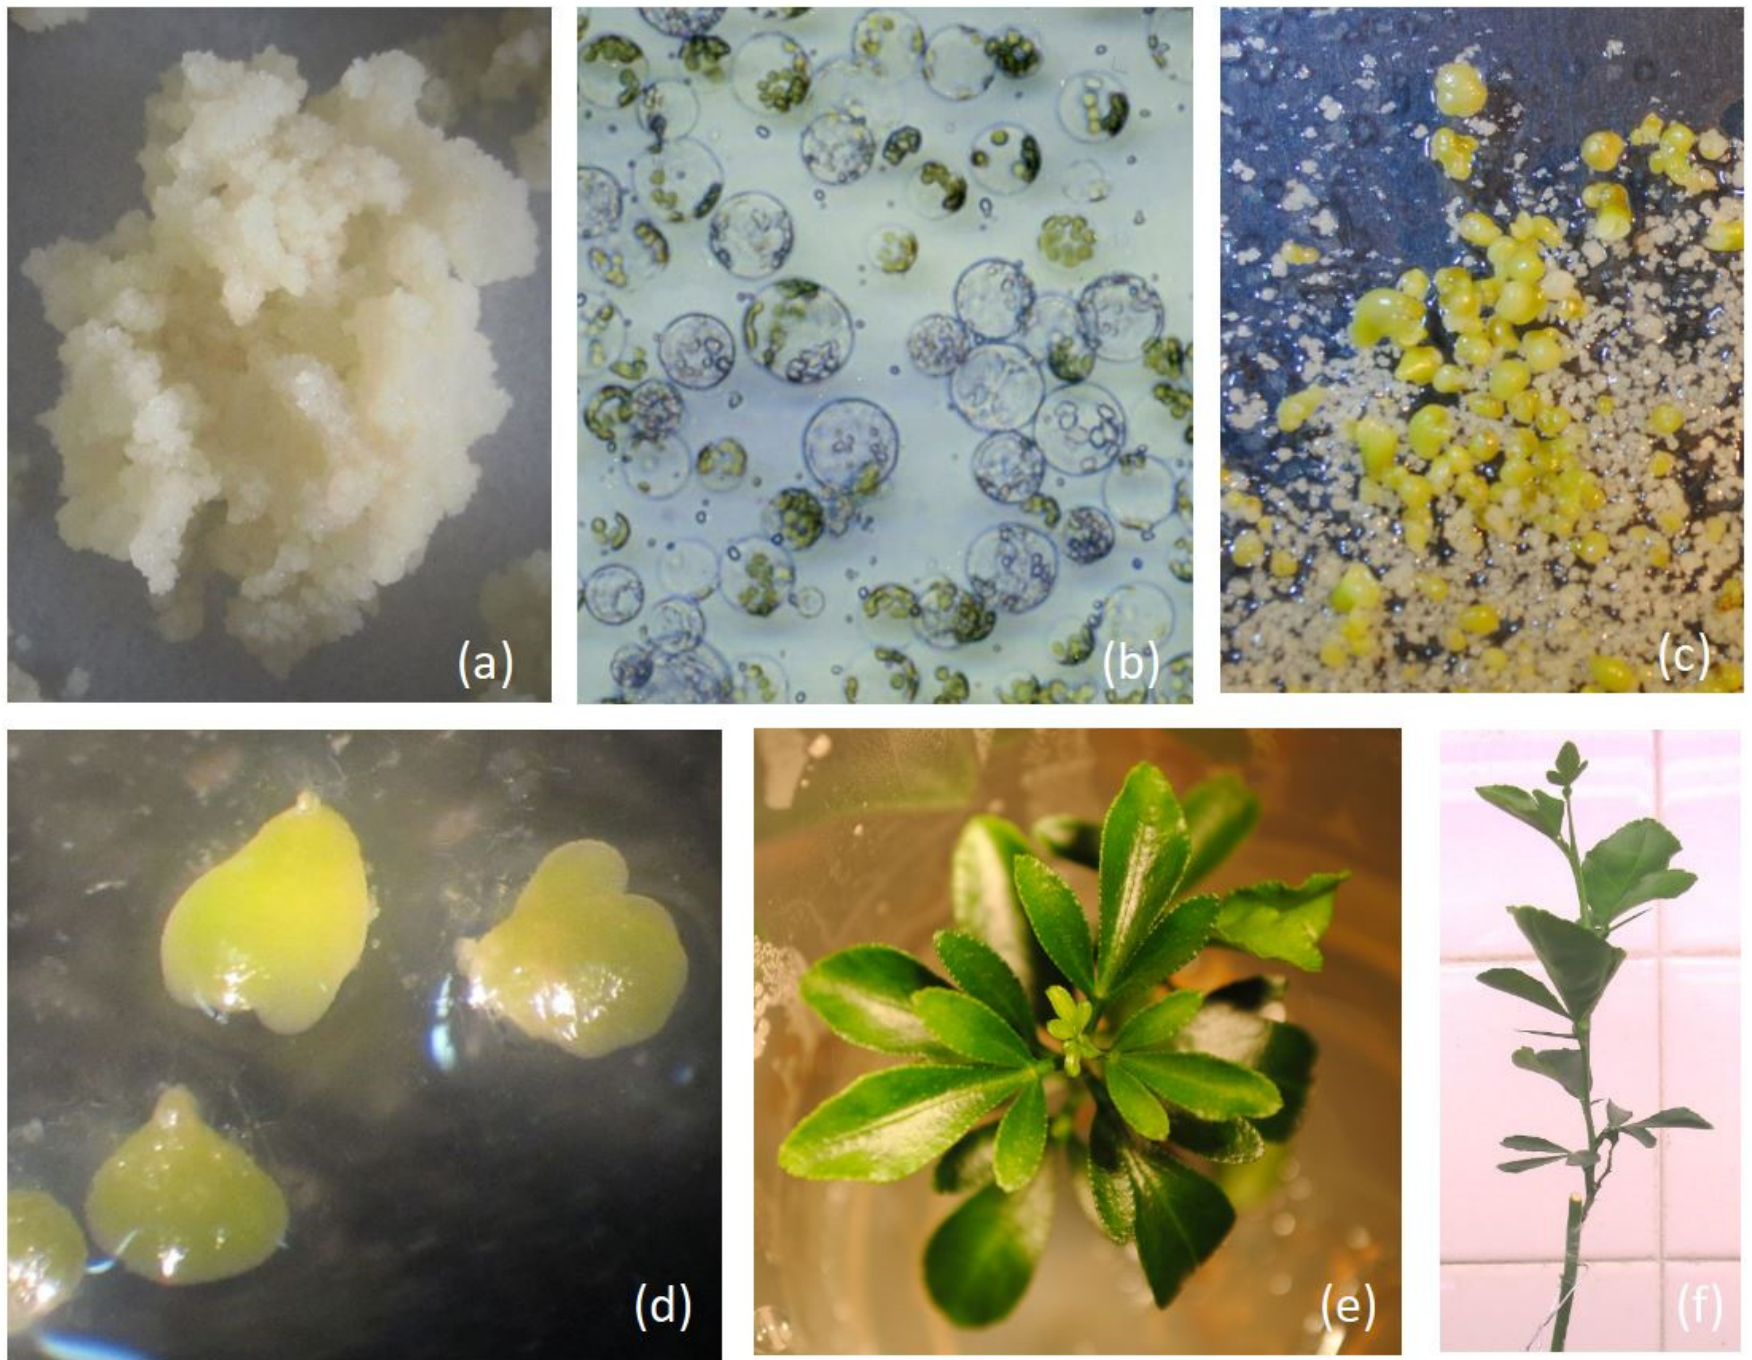
\includegraphics[width=0.6\linewidth]{./../images/protoplast_fusion_citrus_genera} \caption{Process of somatic hybridization and plant regeneration between Citrus and Poncitrus group of plants. (a) embryonic callus line of Shamouti sweet orange; (b) protoplast fused after three pulses (35 micro second) of 220 v (DC); (c) pro-embryo 1 month after fusion; (d) heart shaped embryo two month after fusion; (e) in vitro plantlet of Cleopatra + Winter haven tetraploid somatic hybrid; (f) grafted plant of Shamouti sweet orange + 4475 citrumelo-Chios cybrid tetraploid somatic hybrid. (For more details refer to \url{https://doi.org/10.3390/agriculture12020134})}\label{fig:protoplast-fusion}
\end{figure}
\end{frame}

\hypertarget{genetic-transformation}{%
\section{Genetic transformation}\label{genetic-transformation}}

\begin{frame}{Agrobacterium mediated transformation}
\protect\hypertarget{agrobacterium-mediated-transformation}{}
\end{frame}

\hypertarget{wide-hybridization}{%
\section{Wide hybridization}\label{wide-hybridization}}

\begin{frame}{}
\protect\hypertarget{section-15}{}
\begin{itemize}
\tightlist
\item
  Search for desired genes should start from among materials in the
  primary gene pool (related species), then proceed to the secondary
  gene pool and, if necessary, the tertiary gene pool.
\item
  Crossing involving materials outside the cultivated species is
  collectively described as wide crosses.

  \begin{itemize}
  \tightlist
  \item
    cross involves another species -- interspecific cross (e.g., kale)
  \item
    cross involves a plant from another genus -- intergeneric cross
    (e.g., wheat).
  \end{itemize}
\item
  Crosses between crops with their wild progenitor species should not be
  considered wide crosses, since, despite the sometimes used different
  scientific names (barley \emph{Hordeum vulgare} was derived from
  \emph{H. spontaneum}; lettuce \emph{Lactuca sativa} was derived from
  \emph{L. serriola}). Genetically such ``species'' are fully compatible
  and behave genetically as an intraspecific cross (i.e.~cross within
  the same species).
\end{itemize}
\end{frame}

\begin{frame}{}
\protect\hypertarget{section-16}{}
\begin{figure}
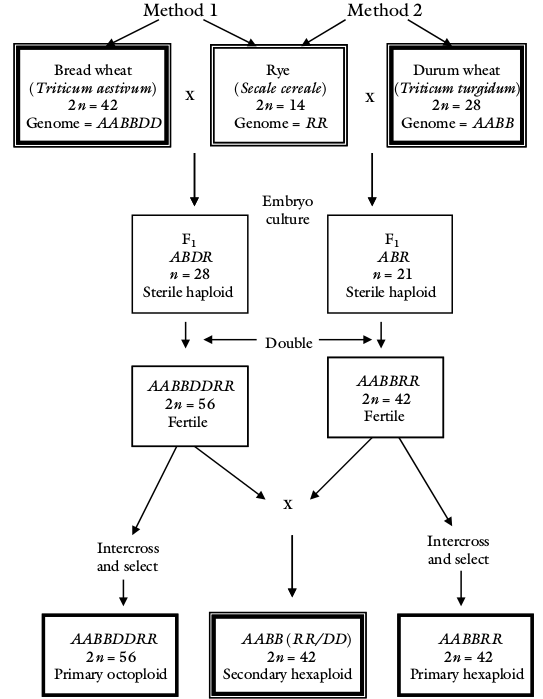
\includegraphics[width=0.35\linewidth]{../images/triticale-development} \caption{Generation of Triticale made possible by wide hybridization between individuals of different genera.}\label{fig:triticale-development}
\end{figure}
\end{frame}

\begin{frame}{Objectives of wide crosses}
\protect\hypertarget{objectives-of-wide-crosses}{}
\begin{itemize}
\tightlist
\item
  Economic crop improvement
\item
  New character expression
\item
  Creation of new allploids (refer to following pages)
\item
  Scientific studies
\item
  Curiosity and aesthetic value
\end{itemize}
\end{frame}

\begin{frame}{}
\protect\hypertarget{section-17}{}
\begin{figure}
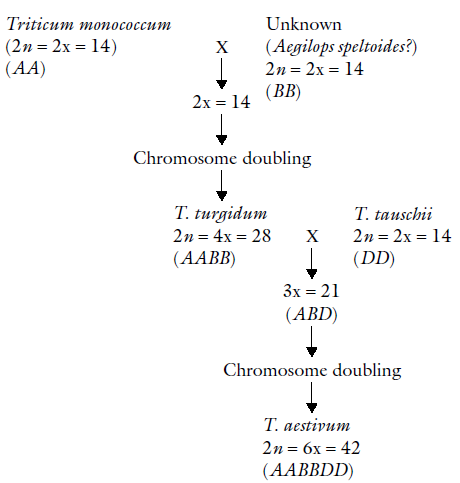
\includegraphics[width=0.45\linewidth]{../images/wheat_ploidy} \caption{Genome evolution of modern \textit{Triticum aestivum} wheat -- a natural allopolyploid derived from wide hybridization. It's lineage can be traced back to at least three distinct ancestor groups.}\label{fig:wheat-evolution}
\end{figure}
\end{frame}

\hypertarget{somaclonal-variaiton}{%
\section{Somaclonal variaiton}\label{somaclonal-variaiton}}

\begin{frame}{}
\protect\hypertarget{section-18}{}
\begin{itemize}
\tightlist
\item
  In vitro culture of plants is supposed to produce clones (genetically
  identical derivatives) from the parent material.
\item
  Tissue culture environment has been known to cause heritable variation
  called somaclonal variation.
\item
  Sometimes variation \emph{in vitro} can be epigenetic (result of
  environmental factors), which cannot be transferred through seed
  progeny.
\item
  Causes include karyotypic changes, cryptic chromosomal rearrangements,
  somatic crossing over and sister chromatid exchange, transposable
  elements, and gene amplification.
\item
  Some of these variations have been stable and fertile enough to be
  included in breeding programs.
\item
  Geenerally used for inducing genetic changes for cold/salt tolerance,
  insect resistance, and new plant forms.
\end{itemize}
\end{frame}

\begin{frame}{}
\protect\hypertarget{section-19}{}
\begin{itemize}
\tightlist
\item
  Growing points like the shoot tips or axillary buds have the least
  chance of mutation.
\item
  Adventitious shoot formation (as opposed to axillary shoot formation),
  callus, and cell suspensions have the greatest chance for genetic
  mutations because they are not genetically stable.
\item
  Long-term cultures and cultures that are forced to grow quickly have
  greater prossibilities of mutation.
\item
  Media with high levels of cytokinins and auxins, especially 2,4-D face
  genetic instability.
\end{itemize}
\end{frame}

\begin{frame}{}
\protect\hypertarget{section-20}{}
\begin{itemize}
\tightlist
\item
  If cloning is the objective of micropropagation, this form of
  variation is undesirable.
\end{itemize}
\end{frame}

\hypertarget{bibliography}{%
\section*{Bibliography}\label{bibliography}}
\addcontentsline{toc}{section}{Bibliography}

\begin{frame}{Bibliography}
\hypertarget{refs}{}
\begin{cslreferences}
\leavevmode\hypertarget{ref-ake2007effect}{}%
Aké, A Pech, B Maust, A Orozco-Segovia, and C Oropeza. 2007. ``The
Effect of Gibberellic Acid on the in Vitro Germination of Coconut
Zygotic Embryos and Their Conversion into Plantlets.'' \emph{In Vitro
Cellular and Developmental Biology-Plant} 43 (3): 247--54.

\leavevmode\hypertarget{ref-sarasan2002vitro}{}%
Sarasan, V, M Ramsay, and A Roberts. 2002. ``In Vitro Germination and
Induction of Direct Somatic Embryogenesis in'Bottle Palm'{[}Hyophorbe
Lagenicaulis (L. Bailey) He Moore{]}, a Critically Endangered Mauritian
Palm.'' \emph{Plant Cell Reports} 20 (12): 1107--11.
\end{cslreferences}
\end{frame}

\end{document}
